%\documentclass[11pt, a4paper, useAMS,usenatbib]{mn2e}
%\documentclass[usenatbib]{mn2e}
\documentclass[useAMS,usenatbib]{mn2e}

%define general packages
%\usepackage{epsfig}
\usepackage{amsmath}
%\usepackage{natbib}
%\usepackage{epstopdf}

\usepackage{epsfig}
\usepackage{epstopdf}
\usepackage{lscape} % Allows landscape environment to be used
\usepackage{natbib}
\usepackage{tabularx}
\usepackage{multirow}
\usepackage{amssymb}
\usepackage{gensymb}

\def\gtrsim{\mathrel{\hbox{\rlap{\hbox{\lower4pt\hbox{$\sim$}}}\hbox{$>$}}}}


\title{FRB repetition and non-Poissonian statistics}
\author[Connor et al.]{
Liam Connor$^{1,2,3}$\thanks{E-mail:\ connor@astro.utoronto.ca}
Ue-Li Pen $^{1, 6, 7}$\thanks{E-mail:\ pen@cita.utoronto.ca}
\\
$^1$ Canadian Institute for Theoretical Astrophysics, University of Toronto, M5S 3H8 Ontario, Canada
\\
$^2$ Department of Astronomy and Astrophysics, University of Toronto, 
M5S 3H8 Ontario, Canada
\\
$^3$ Dunlap Institute for Astronomy and Astrophysics, University of Toronto,
Toronto, ON M5S 3H4, Canada
\\
$^6$ Canadian Institute for Advanced Research, Program in Cosmology
and Gravitation
\\
$^7$ Perimeter Institute for Theoretical Physics, 31 Caroline St. N., Waterloo, ON, N2L 2Y5, Canada
}


\begin{document}
\date{\today}
\pagerange{\pageref{firstpage}--\pageref{lastpage}} 
\pubyear{2015}
\maketitle
\label{firstpage}

\begin{abstract}
We discuss some of the claims that have been made regarding the statistics of 
fast radio bursts (FRBs). We show how if their repeat rate were non-Poissonion
and had some associated flicker noise then the current limits of repetition ($\le$ daily)
would be weakened. The repeat rate has implications for observing strategy, favouring 
shallow wide-field surveys in the case where bursts repeat regularly. 
We also discuss the statistics of the apparent latitudinal dependence of FRBs, which 
is also affected by repetition. We show that the non-uniformity of bursts on the sky
cannot be ruled out with N-$\sigma$, as has been claimed. 

\end{abstract}
\begin{keywords}
\end{keywords}

\newcommand{\be}{\begin{eqnarray}}
\newcommand{\ee}{\end{eqnarray}}
\newcommand{\beq}{\begin{equation}}
\newcommand{\eeq}{\end{equation}}

\section{Introduction}
There is mounting evidence that the new class of transients 
known as fast radio bursts (FRBs) are of astronomical origin.
The most striking features of FRBs are their large dispersion
measures (DMs) -- too high to be attributed to our own Galaxy's
ISM --
and their event rate (10$^3-10^4$ sky$^{-1}$ day$^{-1}$). They
last for $\sim$millisecond with peak flux of $\sim$Jy, and none
has been conclusively shown to repeat. This has lead to the 
interpretation that FRBs are cosmological,
since the intergalactic medium (IGM) would naturally provide
DMs between $\sim$300-1600 pc cm$^{-3}$ for sources at 
$z\sim0.3-1$. 

Given their apparent phenomenological richness
(polarization, scattering, etc.) and considering
how little we know about their location and physical 
origin, it is likely that FRBs will be of interest to the community for 
years to come, assuming they are not terrestrial.
Though we are in the regime of only $\sim$dozen published FRBs, 
at present the conventional wisdom is that they are likely cosmological
in origin \citep{2013Sci...341...53T}, they seem to not repeat regularly
\citep{2015MNRAS.454..457P}, and there is a dearth of bursts 
at low galactic latitudes \citep{2014ApJ...789L..26P, 2014ApJ...792...19B, 2015MNRAS.451.3278M}.
There have been 
a number of models proposed to describe this cataclysmic, cosmological 
scenario \citep{2012ApJ...760...64M, 2013PASJ...65L..12T, 2014A&A...562A.137F, 2015ApJ...814L..20M}.
However since the field is still in its infancy it is important to
leave as many conceptual doors open as possible;
assumptions about the statistics of their event rate, 
spatial distribution, and repetition are important for the design
and observing strategy of upcoming surveys. In section \ref{repeat} we explore the 
consequences of repeating FRBs in the case where their 
burst rate is non-Possionian and exhibits a 1/f power spectrum, 
or pink noise. We also investigate the claims of \cite{2015arXiv150701002M}
that FRB 140514 could have been the same source as FRB 100220, 
and comment on its implications. In section \ref{latitude}
we discuss the statistical treatment of the apparent latitudinal dependence 
of event rate and the lack of detections at low galactic latitude. In section \ref{rate}
discuss the impact of FRB repetition on survey strategy. 

% Usual FRB introduction, swayed towards repetition and statistics.


\section{Repeat rates}
\label{repeat}

Though no source has been shown with certainty to repeat, 
the limits on the repeatability of FRBs are still weak. Several 
models generical predict repetition, whether periodic or stochastic. 
Galactic flaring stars \citep{2015arXiv150701002M}, radio bursting 
magnetars \citep{2007arXiv0710.2006P, 2015ApJ...807..179P}, and pulsar planet systems 
\citep{2014A&A...569A..86M} all predict repetition with varying 
rates and burst distributions. In \cite{2015arXiv150505535C} we 
proposed supergiant pulses from very young pulsars in supernova 
remnants of nearby galaxies could explain the high DMs, Faraday rotation, 
scintillation, and polarization properties of the observed FRBs. We also 
conjecture that if the repetition of supergiant pulses were non-Poissonian 
(with a pink or red distribution) 
then one might expect several bursts in a short period of time.

\subsection{Flicker noise}

Pink noise is ubiquitous in physical systems, showing up in 
geology and meteorology, a number 
of astrophysical sources including quasars and the sun, 
human biology, nearly all electronic devices, finance, 
and even music and speech
\citep{1978ComAp...7..103P, 1975Natur.258..317V}.
Though there is no agreed upon
mathematical explanation for this phenomenon
 \citep{2002physics...4033M}, fluctuations 
are empirically known to be inversely proportional to frequency 
for a variety of dynamical systems.
In the case of a time-domain astronomical 
source, this results in uniformity on short timescales, i.e. a burst of 
clustered events followed by extended periods of quiescence. 
If FRBs were to exhibit such flicker noise then their repetition would 
not only be non-periodic, but would also have a time varying 
burst rate. Therefore the number of events
seen in a follow-up observation would depend strongly on 
the time passed since the initial event.

In \cite{2015MNRAS.454..457P}
the fields of eight FRBs discovered between 2009 and 2013
were followed up from April to October of 2014, for an average 
of $\sim$11.4 hours per field. During this followup programme 
FRB 140514 was found in the same beam as FRB 110220, however
the authors argue that it is likely a new source due to its lower DM. 
After its discovery, the field of 140514 was monitored 
five more times, starting 41 days later on 2014-05-24, without seeing anything.
Under the assumption that 140514 was a new FRB 
that only showed up in the same field 
coincidentally and that the repeat rate is uncorrelated,
 \cite{2015MNRAS.454..457P} rule out repetition with P $\le$ 8.6 
hours and reject 8.6 $<$ P $<$ 21 hours with 90$\%$ confidence.
However it is possible that one or both of those premises 
is invalid, so it is useful to explore the possibility of non-stationary 
repeat rate statistics and repeating FRBs with variable DM. 

If the statistics of the FRB's repeat rate were
non-Poissonian and initial bursts from FRBs were to have aftershocks
similar to earthquakes, then the non-immediate followup observations 
impose far weaker repeat rate limits than has been suggested. We 
constructed a mock followup observation of the eight FRBs whose
fields were observed in \cite{2015MNRAS.454..457P}. We then 
asked how many bursts are seen to repeat if we do an immediate
follow up vs. a followup several years after the initial event 
at times corresponding to 
to those in \cite{2015MNRAS.454..457P}. We Monte Carlo this 
simple simulation with one sample per hour and a probability of 0.5 
that a given sample has a burst in it. 
In the stationary Poisson case, the rate of bursts in 
the immediate followup is the same as the multi-year followup 
since all times are 
uncorrelated. When we use a spectrum of events to be described by 
a 1/f powerlaw, we see $\sim$20$\%$ more events in the case where we
stay on the source after first observing it than when the followup takes 
place several months or years later.

\begin{figure}
  \centering
   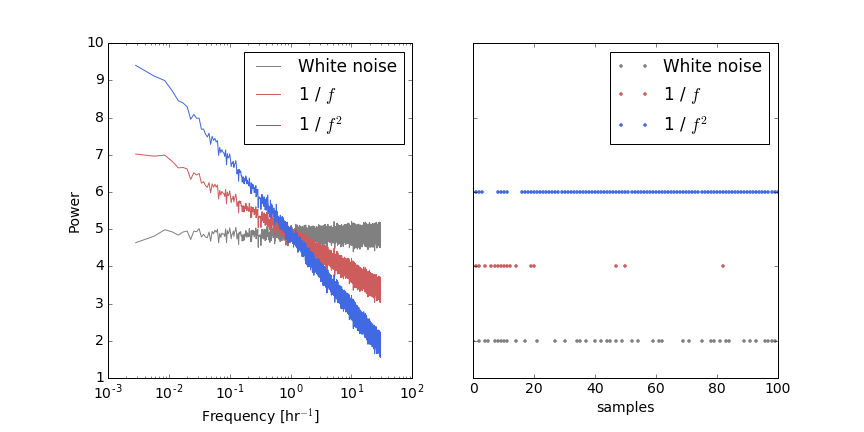
\includegraphics[trim={.5in, 0in, .5in, 0in}, width=0.5\textwidth, height=0.27\textwidth]{frb_sim_pink.png}
   \caption{\textit{left panel}: Power spectrum for pulse arrival times of a single FRB.
   Grey shows a flat spectrum, corresponding to the often assumed Poissonian 
   repetition rate. The red and blue spectra show flicker noise, with pink (1/$f$) 
   noise and Brownian (1/$f^2$) noise respectively. \textit{right panel}: 
   Repeat events following an initial burst for the three different spectra. The average 
   probability of a burst in this simulation is 0.5, which is why roughly half of the 
   bins in the white case have events. In the 1/$f^\alpha$ cases the initial event 
   is followed by a number of pulses due to the increased event rate when in an 
   ``on" state.}
   \label{FIG-RATE}
\end{figure}


\subsection{FRBs 110220 and 140514}
Using the event rate of $\sim10^4$ sky$^{-1}$ day$^{-1}$
from \cite{2013Sci...341...53T}, it 
was originally reported that the probability of seeing a 
new FRB in the field of 110220 during the 85 hours of followup 
was $\sim$0.32  
\citep{2015MNRAS.447..246P}. It was then pointed out by \cite{2015arXiv150701002M} 
that this underestimated the coincidence, since FRB 140514
was found in the same pointing as 110220 during the gridded followup, 
and not one of the four other staggered pointings near the field. 
The probability also dropped due to the updated daily event rate,
given the \cite{2013Sci...341...53T} estimate is now thought to likely be high.
Using the rate calculated in \cite{2015arXiv150500834R}, and following
the procedure of \cite{2015arXiv150701002M}, we find the likelihood of 
$\sim$ 0.25-2.5$\%$. Given the relatively low probability of finding 
a new FRB in the same field and since there are models that predict
burst repetition with variable DMs \citep{2015arXiv150505535C, 2015arXiv150701002M}
one can then ask the question: If one FRB out of eight is found to
repeat during 85 hours of followup, what are the limits on the expected
repeat rate? 


\section{Latitudinal dependence}
\label{latitude}
There is now evidence that the FRB rate is nonuniform on the sky, 
with fewer detectible events at low galactic latitudes \citep{2014ira..book.....B}.
However the statistical significance of this finding may be 
overstated and some of the initial claims premature. In \cite{2014ApJ...789L..26P}
the authors compute the probability of the disparity between the number of 
bursts seen in the the high and low latitude components of the High Time Resolution Universe survey 
(HTRU). They calculate the probability of seeing N=0 in the low-lat survey and M=4 in 
the high-lat, despite having searched 88$\%$ more data in the latter. We would point out 
that in general P(N$|$M) describes a very specific outcome, and P($\le$N$|\ge$M) would be 
more appropriate since it includes all outcomes equally or more unlikely.
That number might also be multiplied by two, since if the survey found 
four low-latitude FRBs and zero high-lat ones, we would ask the same question. HTRU 
has since reported five more bursts in the high galactic region, but using a dataset 
that spent $\sim$2.5 times more time at high-lat. Below we try and quantify the likelihood of 
this.

If one wants to 
test a statistical hypothesis, then that claim should be treated as true and one should
ask with what confidence it can be rejected. 
In the case of testing the abundance of FRBs at high latitudes,
the sky should be bifurcated into high and low regions a priori 
(e.g. the predefined high-lat HTRU and its compliment). The rate in both regions 
is then taken to be the same, and the likelihood of a given spatial distribution of observed
sources can be calculated.
This situation is naturally
described by a biased binomial distribution with a fixed number of events. Suppose
K FRBs are observed in a given survey. We then ask the question, what is the probability of 
seeing M events in the high region and (K-M) events in the lower region? 
This probability can be calculated % Should I include >M in one region?
as 

\begin{equation}
\label{eq-binomial}
\textup{P(M} | \,\textup{K}, p) = \left ( \frac{\textup{K}}{\textup{M}} \right ) p^{\textup{M}} (1-p)^{\textup{K}-\textup{M}} 
\end{equation}

\noindent where $p$ is the probability that an event happens to show up in the 
northern region. In a survey where more time is spent on one part of the 
sky than the other, $p=\alpha \, /(1 + \alpha)$, where $\alpha$ is the ratio of 
time spent in the high-lat region vs. the low region. In the case of the HTRU 
survey, K=9 and since none were found 
in the low-lat region, M=9. Roughly 2500 hours were spent searching the upper region
and $\sim1000$ hours were spent at $|b| < 15\degree$, giving $\alpha=2.5$. Using equation 
\ref{eq-binomial}, this outcome is only 13$\%$ unlikely. 




\section{Event rates and total number of sources}
\label{rate}

If FRBs were found to repeat, their statistics and the
average frequency of their repetition 
should affect the search strategy of upcoming surveys. 
For instance, if it were found that FRBs repeated,
on average, five times a day, then the number of unique 
sources would be five times smaller than the per-sky 
daily event rate. This means the rate 
$3.3^{+5.0}_{-2.5}\times10^3$ sky$^{-1}$ estimated by 
\cite{2015arXiv150500834R} would be produced by
only $\sim$160-1600 sources. In this scenario 
there is no FRB in almost every pixel on the sky, which means
one could integrate on most patches forever without 
seeing an event. Therefore deep surveys are at a disadvantage 
to those that sweep large regions of the sky 
(CHIME  \citep{2014SPIE.9145E..22B}, 
UTMOST\footnote{http://www.caastro.org/news/2014-utmost}, HIRAX)
because the non-repeating 
scenario is unaffected; shallow observations 
should not hurt the detection rate, no matter what their repetition. 
Ideally, a survey
needs only to spend a few dispersion delay times on each beam 
before moving on. 


\section{Conclusions}



\section{Acknowledgements}


\newcommand{\araa}{ARA\&A}   % Annual Review of Astronomy and Astrophys.
\newcommand{\afz}{Afz}       % Astrofizica
\newcommand{\aj}{AJ}         % Astronomical Journal
\newcommand{\azh}{AZh}       % Astronomicekij Zhurnal
\newcommand{\aaa}{A\&A}      % Astronomy and Astrophysics
\newcommand{\aas}{A\&AS}     % Astronomy and Astrophys. Supplement Series
\newcommand{\aar}{A\&AR}     % Astronomy and Astrophysics Review
\newcommand{\apj}{ApJ}       % Astrophysical Journal
\newcommand{\apjs}{ApJS}     % Astrophysical Journal Supplement Series
\newcommand{\apjl}{ApJ}      % Astrophysical Journal Letters
\newcommand{\apss}{Ap\&SS}   % Astrophysics and Space Science
\newcommand{\baas}{BAAS}     % Bulletin of the American Astron. Society
\newcommand{\jaa}{JA\&A}     % Journal of Astronomy and Astrophysics
\newcommand{\mnras}{MNRAS}   % Monthly Notices of the Roy. Astron. Society
\newcommand{\nat}{Nat}       % Nature
\newcommand{\pasj}{PASJ}     % Publ. of the Astron. Society of Japan
\newcommand{\pasp}{PASP}     % Publ. of the Astron. Society of the Pacific
\newcommand{\paspc}{PASPC}   % Publ. Astron. Soc. Pacific Conf. Proc.
\newcommand{\qjras}{QJRAS}   % Quart. Journal of the Royal Astron. Society
\newcommand{\sci}{Sci}       % Science
\newcommand{\solphys}{Solar Physics}       % 
\newcommand{\sova}{SvA}      % Soviet Astronomy
\newcommand{\aap}{A\&A}
\newcommand\jcap{{J. Cosmology Astropart. Phys.}}%
\newcommand{\prd}{Phys. Rev. D}

%\bibliography{frb}
\bibliography{frb_statistics}
\bibliographystyle{mn2e}


\label{lastpage}


\end{document}


